% Chapter X

\chapter{Experiment Website} % Chapter title
\label{ch:website} % For referencing the chapter elsewhere, use \autoref{ch:name} 

%----------------------------------------------------------------------------------------
\section{Experiment Walkthrough}
\label{sec:walkthrough}

\noindent A detailed walkthough of the experiments with screenshots is presented in \autoref{an:walkthrough}. The following subsections provide a more detailed description of the technical side of the server setup (\autoref{sec:server_setup}), how participants found out about the experiment (\autoref{sec:access}), the StyleCheck user interface (\autoref{sec:hint_ui}) and the data that was logged (\autoref{sec:logging}).

%----------------------------------------------------------------------------------------

\section{Server Setup}
\label{sec:server_setup}

\noindent The website where participants carried out the translation tasks was created specifically for this experiment. The website was built using the Flask\footnote{\url{http://flask.pocoo.org/}} (v. 10.1) web framework and Python (3.4.3) from a virtual environment to help manage package dependencies. The \texttt{html} and \texttt{css} code was put together using Bootstrap\footnote{\url{http://getbootstrap.com/}}. The dynamic parts of the user interface were written in \texttt{javascript} using the jQuery\footnote{\url{http://jquery.com/}} library. Using these frameworks, the website was responsive and thus able to be used on mobile devices, although not recommended for this experiment. Despite this recommendation, one participant reported carrying out the experiment on an iPad.

The server ran Ubuntu 12.04 and was set up with nginx\footnote{\url{http://nginx.org/}} (v. 1.9.0) as the front-end reverse proxy and uWSGI\footnote{\url{https://github.com/unbit/uwsgi}} (v. 2.0.10) as the application server communicating with Flask through the \spacedlowsmallcaps{WSGI} protocol\footnote{\url{https://www.python.org/dev/peps/pep-3333/}}. The server had 16 \spacedlowsmallcaps{GB} of \spacedlowsmallcaps{RAM}, 8 \spacedlowsmallcaps{CPU}s and 40 \spacedlowsmallcaps{GB} of \spacedlowsmallcaps{SSD} disk.

\graffito{Note: Due to the embedding of the Google survey form, a large blank space appears in \autoref{fig:web_initial}. Please see \autoref{sec:server_setup} for further explanation.}
The questionnaires were made using Google Forms\footnote{\url{https://www.google.com/forms/about/}} and the results downloaded and analysed as \texttt{.csv} files. Forms created with Google Forms can either be answered by following a link or they can be embedded into a website. For this experiment, the latter option was chosen so as to be less jarring for participants. However, forms can only be embedded into an \mintinline{html}|<iframe>| element. Since some questionnaire pages contained more questions than others, some pages included a lot of blank space in the \mintinline{html}|<iframe>| (see \autoref{fig:web_initial}) while others with more questions had to be scrolled.

%----------------------------------------------------------------------------------------

\section{Experiment Access}
\label{sec:access}

\noindent To access the experiment, participants were requested to contact an email address provided in the Call for Participation announcement. Then, they were provided with a unique link from which to access the experiment. The link \spacedlowsmallcaps{URL} included a unique Participant \spacedlowsmallcaps{ID}, which identified the participant throughout the experiment, and a unique text-setup combination. This enabled the experiment to be carried out with all the possible number of combinations for texts and setups. For example, the \spacedlowsmallcaps{URL} \texttt{www.dvh.io/main/420/123} indicates that the Participant \spacedlowsmallcaps{ID} is 420, Text 1 should be used in the \scratch setup, Text 2 in the \ac{PE} setup and Text 3 in the \style setup.

%----------------------------------------------------------------------------------------

\section{StyleCheck User Interface}
\label{sec:hint_ui}

\noindent The third setup interacted dynamically with the server to show participants style hints as they translated. Every time a \mintinline{html}|<textarea>| where translations where input lost focus, the contents were sent to the server, analysed using StyleCheck, and any style rules parsed sent to the participant's browser. Before sending them, the hints were checked for duplicates (some hints could be generated multiple times in a parse) and if any were found only one instance of the rule was returned. The rules then showed up in a red panel below the corresponding sentence that was parsed (\autoref{fig:hints}).

\begin{figure}[h]
\myfloatalign
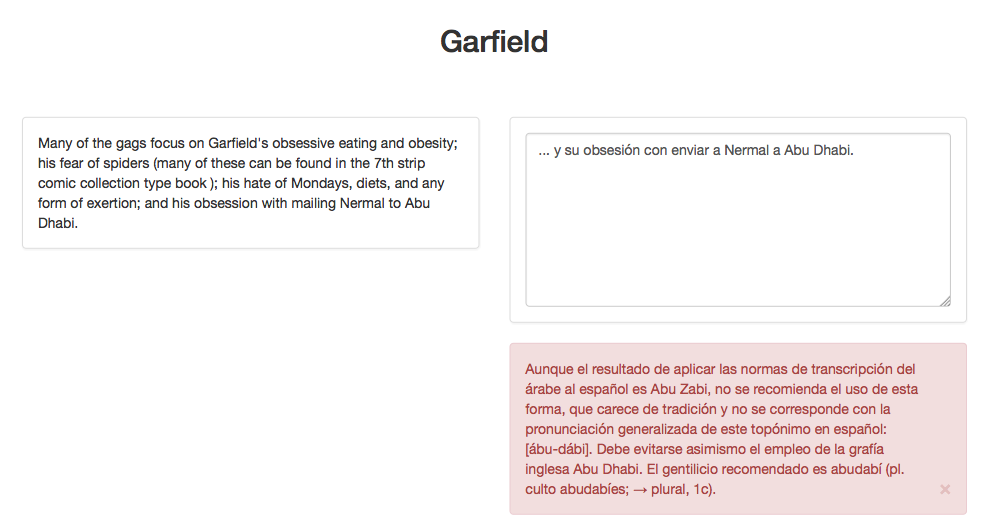
\includegraphics[width=\textwidth]{img/hints/hints.png}
\caption{Hints being shown to the participants after analysing their translations with StyleCheck.}
\label{fig:hints}
\end{figure}

In some cases, due to the length and number of the hints, the panels could take up a lot of space.  Depending on the size of the participant's display and the size of the browser window, the hints could even be rendered outside the visible part of the screen, requiring participants to scroll (\autoref{fig:hints_long}).

\begin{figure}[!ht]
\myfloatalign
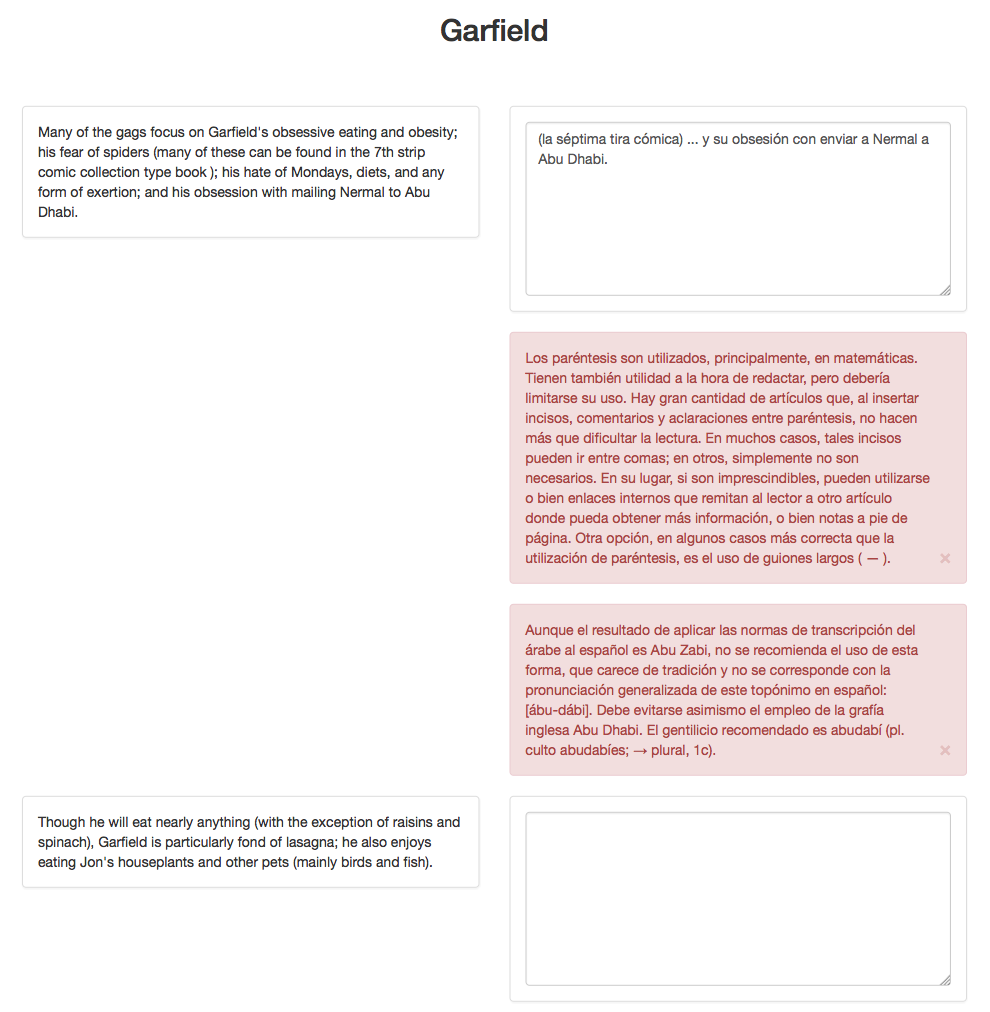
\includegraphics[width=\textwidth]{img/hints/hints_long.png}
\caption{Two long hints being shown taking up a large part of the screen.}
\label{fig:hints_long}
\end{figure}

%------------------------------------------------

\section{Logging}
\label{sec:logging}

\noindent Different kinds of logging, in addition to saving the final translations, were set up in the server:

\begin{itemize}
\item \textit{Style guide click}: When a participant clicked on the link to Wikipedia's style guide, the page the participant was on (the translation brief is shown on four different pages, see \autoref{an:walkthrough}) and the click time was registered.
\item \textit{Translation information}: The website saved the actual translation, as well as the start and end time for each setup.
%\item \textit{Key activity logging}: The website recorded when a key was pressed within the \mintinline{html}|<textarea>| elements where participants wrote in their translations. Both the time and key was recorded. Due to a lack of time, key activity for special keys (backspace, shift, etc.) were not able to be recorded, although the moment when one was pressed was logged. Thus, the logged data should only be considered useful to track key-press activity and not the actual keys themselves.
\item \textit{Hints}: For the \style setup, the contents of the \mintinline{html}|<textarea>| element, the time and any style hints returned were logged.
\end{itemize}


%----------------------------------------------------------------------------------------

